\section {Implementation}

We implemented MindMargin as a classical client/server web-application. Users interact with the MindMargin client as a frontend system using a web browser. The client communicates with the server backend using AJAX to a) request existing data or b) persist new data. The server reads and stores data in a relational database.

\subsection{Frontend}
The client interface consists of a clean user interface to avoid design cluttering and distraction. Figure \ref{fig:frontend} shows the MindMargin system in action. The application is split into two sides: The reference media appears on the left while the actual commenting system appears on the right. The commenting system includes a horizontal infinite scroll component. Thus, a non-restricted amount of comments can be linked to the reference media. Navigation within the infinite scroll component can be performed via mousewheel interaction (either left/right or top/down scrolling with the same effect) or via a slider on the bottom of the screen. For visual orientation, comments are anchored to elements of the reference media by thin lightgray lines. Replies to comments appear on click to, again, enhance user focus. While navigating through comments, the reference media sticks to the left for quick reference.

\begin{figure}
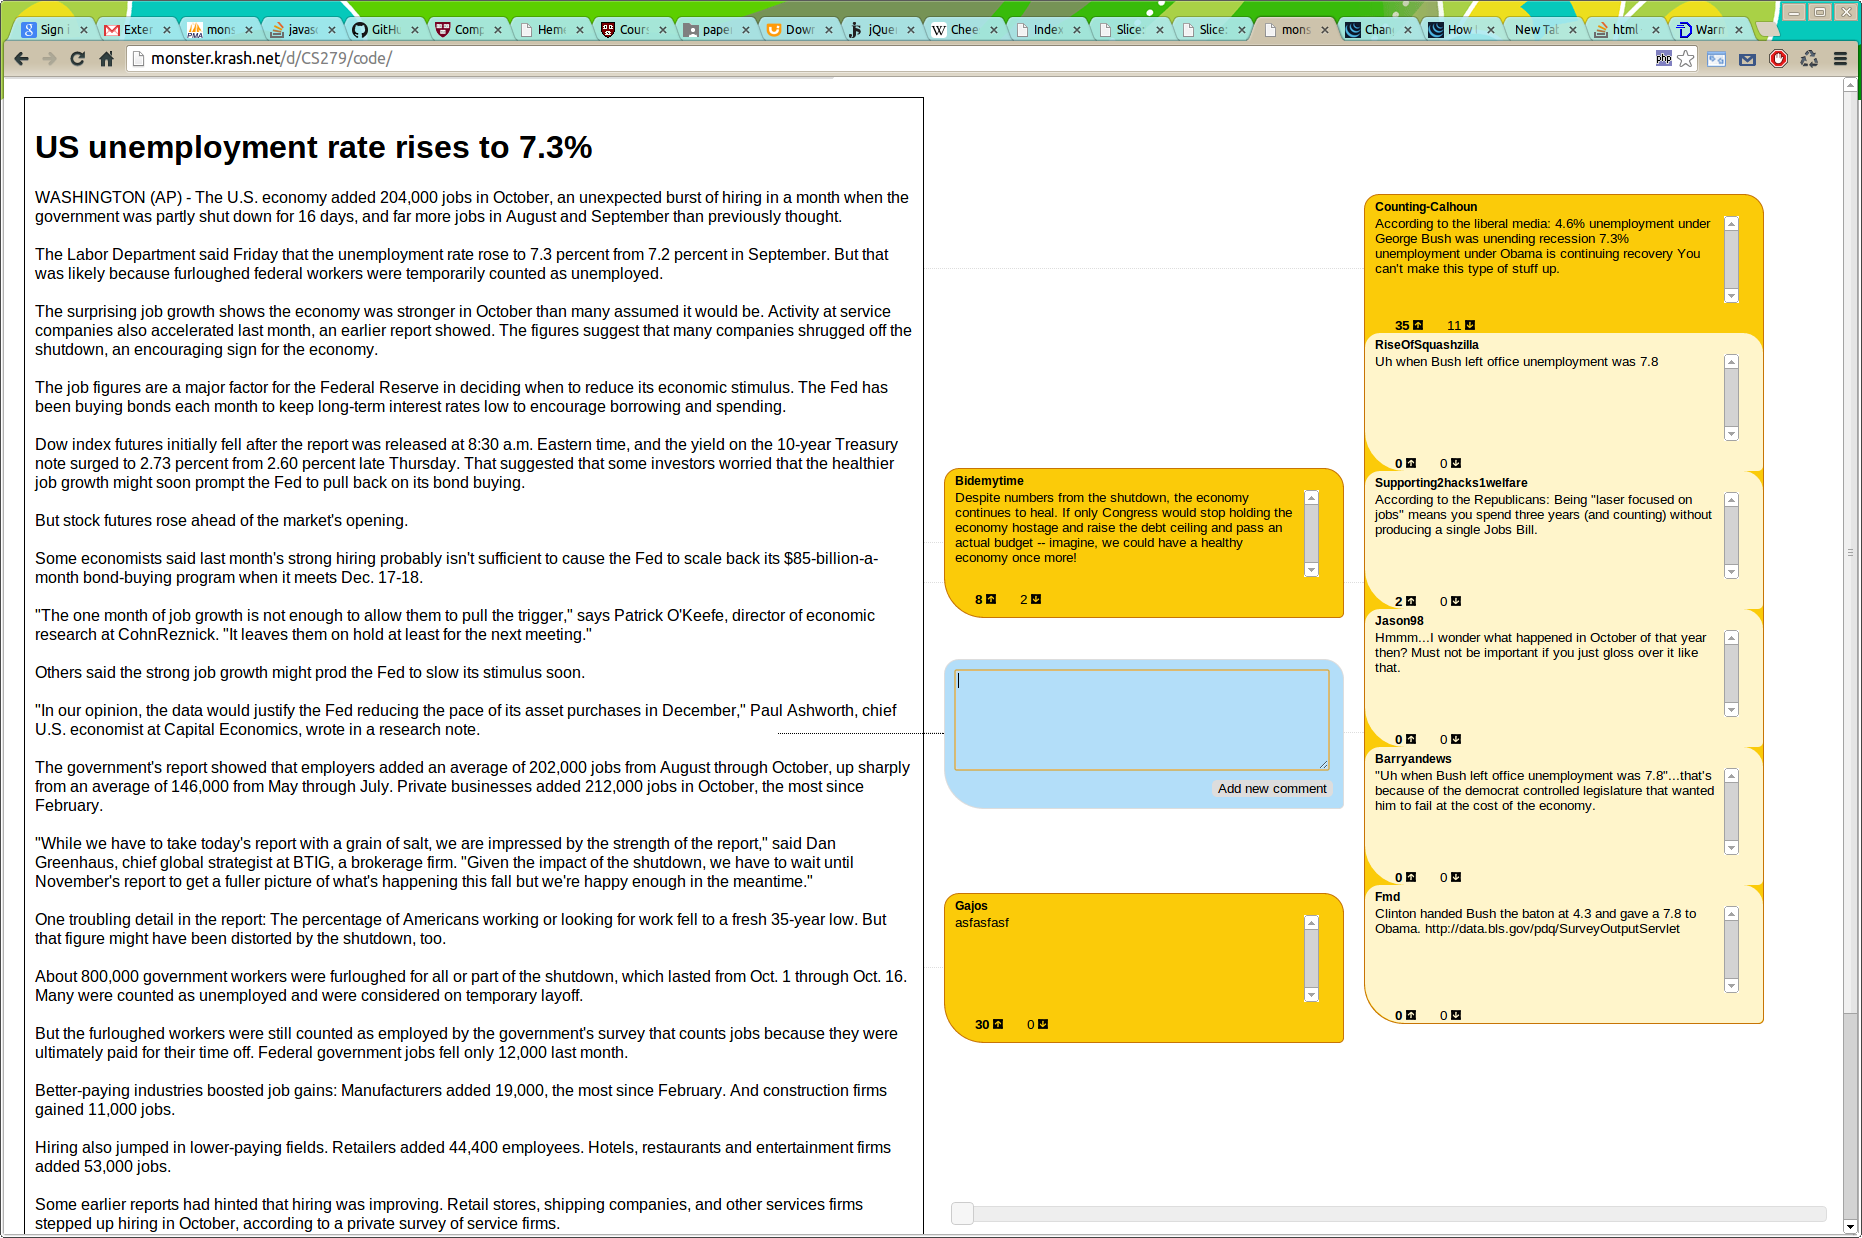
\includegraphics[scale=0.13]{mindmargin.png} 
\caption{The MindMargin system consists of a web client (shown here) and a server side backend.}
\label{fig:frontend}
\end{figure}


The MindMargin frontend was written in JavaScript using the popular jQuery and jQuery UI libraries. A model-view-controller pattern was chosen to structure the application code base. The user interface itself was created as a responsive design to function with any window size.

\subsection{Backend}
The server component of MindMargin was written in PHP and communicates with the frontend and a relational database. Communication with the frontend is ensured by providing a REST-API which can be called via AJAX. The entity model of the client is replicated on the server and we read and store data using a custom and fully generalized object-relational-mapper. We chose MySQL as the database solution and use a comment and a user table.

Throughout the implementation we followed an iterative approach in an extreme programming fashion. The developer team was small. All developed code is released under the BSD open source license on github.